 %iffalse
\let\negmedspace\undefined
\let\negthickspace\undefined


\documentclass[journal,12pt,onecolumn]{IEEEtran}
\usepackage{cite}
\usepackage{amsmath,amssymb,amsfonts,amsthm}
\usepackage{graphicx}
\usepackage{textcomp}
\usepackage{xcolor}
\usepackage{hyperref}
\usepackage{mathtools}
\usepackage{gensymb}
\usepackage{tkz-euclide} 
\newcommand{\myvec}[1]{\begin{pmatrix} #1 \end{pmatrix}}
\newcommand{\brak}[1]{\left( #1 \right)}

\begin{document}
\bibliographystyle{IEEEtran}

\vspace{3cm}
\title{Solution for Question 1.5.16}
\author{AI24BTECH11035-Preethika}
\maketitle

\begin{enumerate}
    \item Find the coordinates of a point A where AB is a diameter of the circle with center (3, -1) and the point B is (2, 6).\\
    
    \textbf{Solution:} Given,\\
    Center of the circle C = (3, -1), and point B = (2, 6).
    
    Let the coordinates of point A be (x, y).  
    Since AB is the diameter of the circle, the center is the midpoint of A and B.
    
    Using the midpoint formula, we have:
    
\[
    \left( \frac{x + 2}{2}, \frac{y + 6}{2} \right) = (3, -1)
\]
    
    This gives two equations:
    
\[
    \frac{x + 2}{2} = 3 \quad \Rightarrow \quad x + 2 = 6 \quad \Rightarrow \quad x = 4
\]
    
\[
    \frac{y + 6}{2} = -1 \quad \Rightarrow \quad y + 6 = -2 \quad \Rightarrow \quad y = -8
\]
    
    Therefore, the coordinates of point A are (4, -8).
    
\end{enumerate}

\begin{figure}[ht]
   \centering
   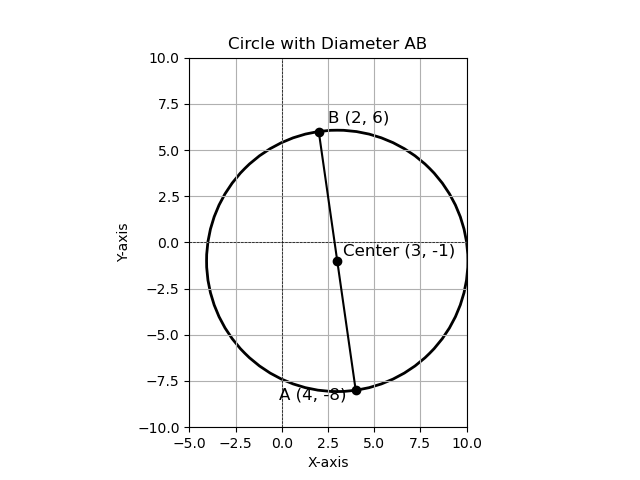
\includegraphics[width=0.7\linewidth]{Figs/fig_1.png}
   \caption{Graph of the Circle with Diameter AB}
   \label{q16}
\end{figure}

\end{document}

